% !TeX program = pdflatex
% One transform and one duality: a machine-checked core of music theory in Lean 4, from
%   pitch-class sets to tuning lattices.  -- the CORPUS PAPER (umbrella of Notes #1/#2/#3).
% Author: Carles Marin (with Claude, Anthropic, as AI assistant).
% Style: HOUSE LINE of the music-math notes, scaled to a full paper -- complete compiling
%   article, question-driven narrative (\question lead-ins, one connecting object per
%   pillar), HONESTY in a dedicated "Novelty, scope, and what this does not claim" section
%   (NOT inline per-theorem tags), Lean theorems in TABLES, TikZ figures, \audio links,
%   \thanks AI-assistant footnote, inline thebibliography. Mirrors sixthirty_note.tex.
% Build: pdflatex corpus_paper.tex (twice, for refs).
% Source of record: research/music-math/CORPUS_PAPER.md (Curiosity, private repo).
% Zenodo DOI: [RESERVE before final compile]. Venue target: MCM (Springer LNCS) -- this
%   article-class build is the working master; an llncs port is the final-format step.
% STATUS: master skeleton in the house line. The three pillar bodies (\input below) are
%   being CONVERTED from the earlier inline-tag drafts to this line (narrative + Lean-in-
%   tables + figures + audio, no inline tags); until converted, compile intro+novelty+
%   frontier standalone by commenting the three \input lines.

\documentclass[11pt]{article}
\usepackage[T1]{fontenc}
\usepackage{lmodern}
\usepackage{amsmath,amssymb,amsthm,booktabs,graphicx}
\usepackage{longtable}
\usepackage[hidelinks]{hyperref}
\usepackage{xurl}
\usepackage[table]{xcolor}
\usepackage[margin=1in]{geometry}
\usepackage{microtype}
\usepackage{float}
\usepackage[section]{placeins}
\usepackage{tikz}
\usetikzlibrary{arrows.meta,positioning,calc}

% two semantic spot colors (meaning is ALSO carried by fill/linestyle -> grayscale-safe)
\definecolor{ctA}{HTML}{1B6F8C} % the autocorrelation / DFT thread, transposition forms
\definecolor{ctB}{HTML}{B5530F} % the duality thread, inversion forms
\setlength{\emergencystretch}{2em}

% --- float placement: let LaTeX pack floats densely so it does not strand whitespace ---
% (the default parameters are conservative; these are the standard "less whitespace" values)
\renewcommand{\topfraction}{0.92}        % up to 92% of a page top may be floats
\renewcommand{\bottomfraction}{0.85}
\renewcommand{\textfraction}{0.07}       % require only 7% text on a mixed page
\renewcommand{\floatpagefraction}{0.78}  % a float-only page must be >=78% full
\setcounter{topnumber}{3}\setcounter{bottomnumber}{2}\setcounter{totalnumber}{5}

\newtheorem{theorem}{Theorem}[section]
\newtheorem{proposition}[theorem]{Proposition}
\newtheorem{lemma}[theorem]{Lemma}
\newtheorem{remark}[theorem]{Remark}
\newtheorem{definition}[theorem]{Definition}

\newcommand{\lean}[1]{\texttt{#1}}
\newcommand{\Ztwelve}{\mathbb{Z}_{12}}
\newcommand{\Zn}[1]{\mathbb{Z}_{#1}}
\newcommand{\Dgrp}[1]{D_{#1}}
\newcommand{\Ahat}{\hat{A}}
\newcommand{\Fi}{\mathcal{F}^{-1}}
\newcommand{\Stab}{\mathrm{Stab}}
% a light "question" lead-in for each section (the connecting thread), as in the notes
\newcommand{\question}[1]{\smallskip\noindent\textit{#1}\smallskip}
% per-example audio links (live on the public repo); accent color so they read as clickable
\newcommand{\audiobase}{https://github.com/karlesmarin/music-math/raw/main/media}
\newcommand{\audio}[1]{\href{\audiobase/#1}{\textcolor{ctA}{\footnotesize\,[$\flat$\,audio]}}}

\title{\bf One transform and one duality\\[5pt]
  \large\rm a machine-checked core of music theory in Lean~4,\\
  from pitch-class sets to tuning lattices}
\author{Carles Mar\'in\thanks{Prepared with the assistance of an AI system (Claude, Anthropic).
The mathematics is classical; every claim, scope statement, and limitation is the author's
responsibility. The boundary of the contribution is stated plainly in
Section~\ref{sec:novelty}, and the Lean~4 kernel---not the assistant---is what certifies the
formalized parts.}\\[3pt]
  \normalsize Independent researcher\\
  \normalsize \texttt{karlesmarin@gmail.com}}
\date{June 2026\\[3pt]\normalsize DOI: \href{https://doi.org/10.5281/zenodo.20953768}{10.5281/zenodo.20953768}\quad\textbullet\quad
  \href{https://github.com/karlesmarin/music-math}{github.com/karlesmarin/music-math}}

\begin{document}
\maketitle

\begin{abstract}\noindent
The mathematics of music theory is real mathematics, but almost all of it lives in prose and
worked examples. We certify its core in Lean~4 on top of Mathlib, over the chromatic universe
$\Ztwelve$, and we organize the library so that one object and one phenomenon do most of the
work. The object is the autocorrelation, or power spectrum $|\Ahat|^2$, of a pitch-class set:
the interval vector, Babbitt's hexachord theorem, homometry and the Z-relation read as the
crystallographic phase problem, deep scales, rhythmic oddity, and the common-tone theorems are
all functions of it, and maximal evenness reconnects to it in the scale theory. The phenomenon
is duality: the neo-Riemannian $PLR$ group is the centralizer of the regular $T/I$ action on
the $24$ triads (Crans--Fiore--Satyendra, via the regular case of Wielandt's centralizer
theorem, a lemma we add over Mathlib), and the same shape recurs as a tritone-centered
order-$12$ self-duality of the Petrushka set class $6$-$30$ and as the val--comma lattice
duality of regular temperament theory. Every theorem is sorry-free with a clean axiom audit.
The underlying mathematics is classical. What we add is the formalization---to our knowledge
the first comprehensive one in this area, since prior proof-assistant work covers only the
$T/I$ action---together with an autocorrelation/DFT organizing lens and two results that
appear not to have been noted in the literature: the $6$-$30$ self-duality and a unified phase
taxonomy of the $|\Ahat|^2$ invariants.
\end{abstract}

\section{Introduction}\label{sec:intro}

\question{What can a proof assistant certify about the mathematics of music---and how much of
it is really one or two ideas seen from many sides?}

Pitch-class set theory, transformational and neo-Riemannian theory, and the theory of scales
and tuning have built, across half a century, a substantial body of mathematics over the cyclic
group $\Ztwelve$, the dihedral group, $\mathbb{Z}$-lattices, and the discrete Fourier transform:
the hexachord theorem, the $Z$-relation, the $T/I$--$PLR$ duality, maximal evenness, the
three-gap theorem, regular temperament theory. The proofs are correct in the ordinary
mathematical sense, but they are \emph{believed} correct, not checked to the standard a kernel
demands; and the literature carries a long tail of near-misses and folklore stated more strongly
than it holds. This paper certifies that core in Lean~4. It is the umbrella over three notes
that appeared separately---on the $6$-$30$ self-duality~\cite{Note1}, the phase
taxonomy~\cite{Note2}, and the Tonnetz spectrum~\cite{Note3}---and it adds the connective tissue
that makes them one library.

\paragraph{What machine-checking buys.} Our motivation is an \emph{honesty floor}. A
machine-checked statement draws a hard line between what is proven and what is merely plausible.
Where a classical argument quietly assumes a non-degeneracy, a formalization must surface it;
where a textbook claim is stated for ``a scale'' but holds only for the diatonic, the Lean
statement names the instance. We treat \textsc{unauditable} as information, not failure: when
only an instance is proven we say so, and we never inflate a first formalization into a claim of
new mathematics. The contribution boundary is drawn in one place, plainly, in
Section~\ref{sec:novelty}; everything outside it is a first formalization of a published theorem.

\paragraph{The model, the substrate, the trust convention.} We work over $\Ztwelve$. A
pitch-class set is a \lean{Finset}\,$\Ztwelve$; a triad is a point of
$\Ztwelve\times\mathrm{Bool}$; a scale is a cyclically ordered tuple. We build on two pieces of
Mathlib verbatim rather than rebuild them: the discrete Fourier transform \lean{ZMod.dft}
(Loeffler~\cite{Loeffler}), which gives $\Ahat$, the power spectrum, inversion and Parseval for
free, and the dihedral group \lean{DihedralGroup}\,$12$, which \emph{is} the group of
transpositions and inversions on the chromatic circle. Every theorem reported here is
sorry-free, and we state its axiom audit: the large majority depend only on
$[\mathrm{propext},\,\mathrm{Classical.choice},\,\mathrm{Quot.sound}]$, the standard Mathlib
base, with no \lean{sorryAx}; the few finite-census results in the scale theory additionally
invoke \lean{native\_decide} and so carry $\mathrm{Lean.ofReduceBool}$, which we flag at each
occurrence while keeping the surrounding analytic engines census-free.

\paragraph{The library at a glance.} For a reader who does not work in Lean, Table~\ref{tab:metrics}
fixes the scale of what ``machine-checked'' means here. The full sources, the Sage/GAP witness
scripts, and the figures are available at \url{https://github.com/karlesmarin/music-math}; every
theorem is checkable with \lean{\#print axioms} and every script is re-runnable.

\begin{table}[H]
\centering\small
\rowcolors{2}{ctA!7}{white}
\begin{tabular}{@{}l r@{}}
\toprule
\rowcolor{ctA!22}
\textbf{Metric} & \textbf{Value}\\
\midrule
Lean source files (the three pillars) & $9$\\
Theorems and lemmas & $275$\\
Total declarations (incl.\ defs, instances) & $372$\\
Lines of Lean & ${\approx}\,3{,}800$\\
\lean{sorry} / \lean{admit} & $0$\\
New lemmas contributed to Mathlib's gap & $1$ (Wielandt, regular case)\\
Dependency & Mathlib (Lean~4)\\
Axiom base & \texttt{propext}, \texttt{Classical.choice}, \texttt{Quot.sound}\\
\bottomrule
\end{tabular}
\caption{The machine-checked library behind the three pillars. Every theorem is sorry-free; the
only departures from the axiom base are the finite \lean{native\_decide} censuses of
\S\ref{sec:p3-me}, which add \lean{Lean.ofReduceBool}.}
\label{tab:metrics}
\end{table}

\subsection{Two recurring ideas}\label{sec:intro-threads}

What makes this one paper rather than a catalogue is that two ideas organize much of it, and
they recur across the three pillars (Figure~\ref{fig:arch}).

\question{Thread~1. What if the interval vector, the hexachord theorem, homometry, deep scales,
rhythmic oddity, common tones, and even maximal evenness are all the same object?}

\noindent\textbf{The autocorrelation / DFT.} A single object---the power spectrum $|\Ahat|^2$,
equivalently the autocorrelation, equivalently the crystallographers' Patterson
function---stands behind a large family of the invariants of Pillar~1 (\S\ref{sec:pillar1}).
These are not analogies: each is a theorem equating the invariant to an inverse DFT of
$|\Ahat|^2$, so that
homometry is \emph{exactly} the loss of phase and the complete transform $\Ahat$ is exactly the
missing completion. The same thread resurfaces in Pillar~3: the maximally even scale is the one
whose interval content extremizes a convex energy---the $|\Ahat|^2$-side maximizer---so the
diatonic's specialness is, once more, a statement about its autocorrelation.

\question{Thread~2. When a group acts simply transitively, it has a dual that is its own
mirror---what does that buy a chord, a symmetric chord, a tuning?}

\noindent\textbf{Duality: simply transitive $\Rightarrow$ self-centralizing.} Lewin's dual pair,
the $T/I$ group and the neo-Riemannian $PLR$ group each the centralizer of the other on the $24$
triads, is the Crans--Fiore--Satyendra theorem of Pillar~2 (\S\ref{sec:pillar2}); its engine is
the regular case of Wielandt's centralizer theorem. The same shape, over a different object,
gives the tritone-centered order-$12$ self-duality of the hexachord $6$-$30$. And it rhymes once
more in Pillar~3, where regular temperament theory pairs the lattice of vals with the lattice of
commas over $\mathbb{Z}$-modules. We point out this rhyme but do not claim a meta-theorem
unifying the group-action and lattice dualities; the two live in different categories, and we
have no such theorem.

\begin{figure}[H]
\centering
\resizebox{\textwidth}{!}{%
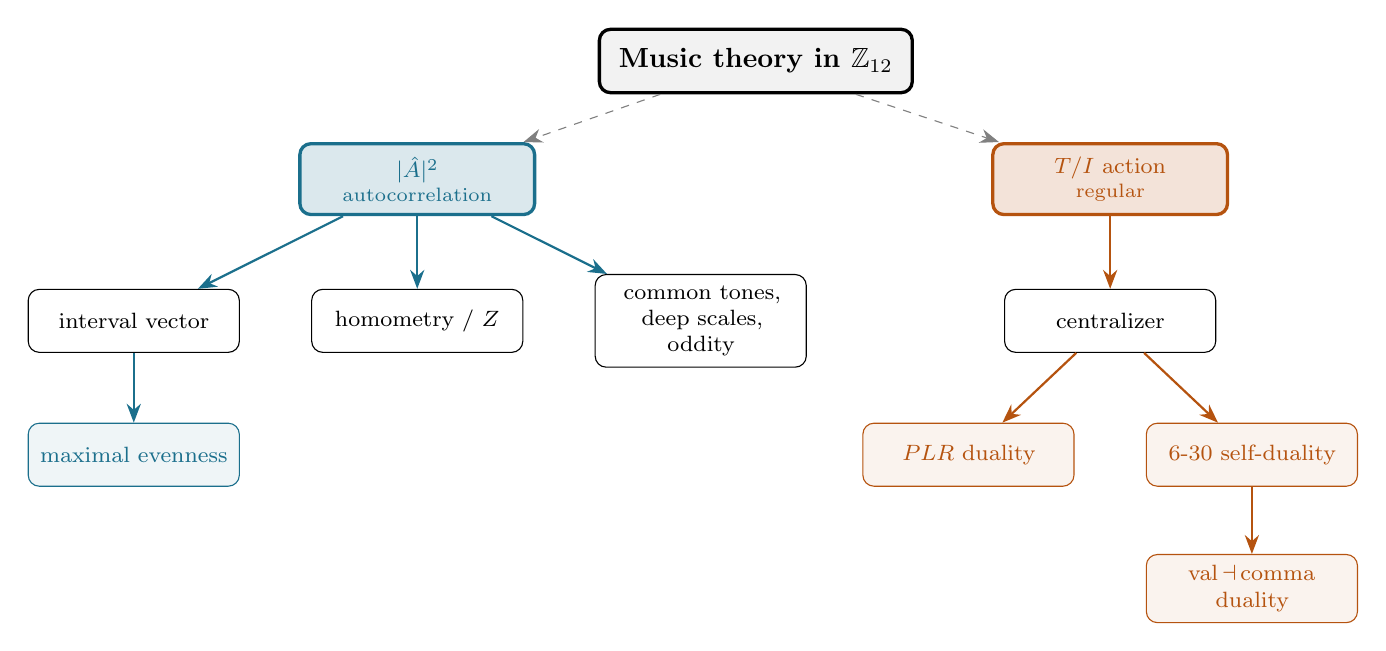
\begin{tikzpicture}[>={Stealth[length=2.4mm]},every node/.style={font=\footnotesize},
    box/.style={draw,rounded corners,inner sep=4pt,align=center,minimum height=8mm,text width=2.4cm},
    root/.style={draw,very thick,rounded corners,inner sep=4pt,align=center,minimum height=9mm,text width=2.7cm}]
  % ---- crown ----
  \node[draw,very thick,rounded corners,fill=black!5,font=\bfseries,inner sep=7pt] (crown) at (5.1,1.5)
       {Music theory in $\Ztwelve$};
  % ---- LEFT tree: the autocorrelation (Thread 1) ----
  \node[root,ctA,fill=ctA!16] (pw) at (0.8,0) {$|\Ahat|^2$\\[-1pt]\scriptsize autocorrelation};
  \node[box] (iv)  at (-2.8,-1.8) {interval vector};
  \node[box] (hom) at (0.8,-1.8)  {homometry / $Z$};
  \node[box] (ct)  at (4.4,-1.8)  {common tones,\\ deep scales, oddity};
  \node[box,ctA,fill=ctA!7] (me) at (-2.8,-3.5) {maximal evenness};
  \draw[ctA,->,thick] (pw)--(iv); \draw[ctA,->,thick] (pw)--(hom); \draw[ctA,->,thick] (pw)--(ct);
  \draw[ctA,->,thick] (iv)--(me);
  % ---- RIGHT tree: the duality (Thread 2) ----
  \node[root,ctB,fill=ctB!16] (ti) at (9.6,0) {$T/I$ action\\[-1pt]\scriptsize regular};
  \node[box] (cen) at (9.6,-1.8) {centralizer};
  \node[box,ctB,fill=ctB!7] (plr) at (7.8,-3.5) {$PLR$ duality};
  \node[box,ctB,fill=ctB!7] (s30) at (11.4,-3.5) {6-30 self-duality};
  \node[box,ctB,fill=ctB!7] (vc) at (11.4,-5.2) {val\,$\dashv$\,comma duality};
  \draw[ctB,->,thick] (ti)--(cen); \draw[ctB,->,thick] (cen)--(plr); \draw[ctB,->,thick] (cen)--(s30);
  \draw[ctB,->,thick] (s30)--(vc);
  % ---- crown connectors ----
  \draw[gray,dashed,->] (crown)--(pw); \draw[gray,dashed,->] (crown)--(ti);
\end{tikzpicture}}
\caption{The thesis in one picture: the formalized core of music theory in $\Ztwelve$ rests on two
mechanisms. \emph{Left} --- the autocorrelation $|\Ahat|^2$ is the common root of the interval
vector, homometry / the $Z$-relation, and the common-tone family (deep scales, rhythmic oddity),
and through the interval vector it reaches maximal evenness (Pillars~1 and~3). \emph{Right} --- a
simply transitive $T/I$ action has a self-centralizing dual, which branches into the $PLR$ duality
of triads and the 6-30 self-duality, the latter continuing to the val\,$\dashv$\,comma duality of
temperament theory (Pillars~2 and~3). The two columns are structurally parallel; we do not claim a
theorem joining them.}
\label{fig:arch}
\end{figure}

\paragraph{The arc.} Pillar~1 (\S\ref{sec:pillar1}) develops the Fourier invariants and closes
at the phase taxonomy. Pillar~2 (\S\ref{sec:pillar2}) develops the $T/I$--$PLR$ duality and the
$6$-$30$ self-duality. Pillar~3 (\S\ref{sec:pillar3}) develops scales and tuning, where the two
threads meet again. Section~\ref{sec:novelty} states plainly what is new versus first
formalization; Section~\ref{sec:frontier} records the open frontier---what we can state but not
yet certify in the kernel.

% ===========================================================================
% The three pillar bodies, in the house line (narrative + Lean-in-tables + figures + audio,
% honesty deferred to Section 5). CONVERSION IN PROGRESS from the inline-tag drafts.
% ===========================================================================
% pillar1_fourier.tex -- Pillar 1 body of corpus_paper.tex, in the HOUSE LINE.
% No preamble: relies on the master's macros (\question, \lean, \audio, \Ahat, \Fi, \Ztwelve,
%   theorem/definition/remark envs, ctA/ctB spot colors). Honesty lives in the master's
%   Novelty section (Sec. \ref{sec:novelty}) -- NO inline tags here. Lean theorems in a table.
% Source of exposition: Note #2 (phase_taxonomy_note.tex); content audited against Fourier.lean
%   and IntervalVector.lean.

\section{Pillar 1: Fourier invariants of pitch-class sets}\label{sec:pillar1}

\question{P\textsubscript{0}. The interval vector, the hexachord theorem, homometry, deep scales,
rhythmic oddity, the common-tone theorem --- what if they are all one object, seen through
different folds?}

Encode a pitch-class set $A\subseteq\Ztwelve$ by its $0/1$ indicator and take its discrete
Fourier transform $\Ahat=\mathcal{F}(\mathrm{ind}\,A)$, built on Mathlib's \lean{ZMod.dft}
(Loeffler~\cite{Loeffler}): $\Ahat(t)=\sum_{a\in A}e^{-2\pi i\,at/12}$ (\lean{Ahat}). Write
$\Ahat=|\Ahat|\,e^{i\varphi}$. The claim of this pillar is that the \emph{power spectrum}
$|\Ahat|^2$ (\lean{powerSpec})---equivalently the autocorrelation, equivalently the
crystallographers' Patterson function---is a single object behind a large family of the classical
invariants, and that the boundary of what it can see is \emph{exactly} the phase $\varphi$. Each
statement below is a theorem in \lean{Fourier.lean}/\lean{IntervalVector.lean}
(Table~\ref{tab:p1}), sorry-free and axiom-clean.

\subsection{The interval vector is the autocorrelation}\label{sec:p1-ivkey}

\question{P\textsubscript{1}. Why is the interval vector invariant under transposition and
inversion---and what is it, spectrally?}

The interval vector counts, for each interval class $k$, the ordered pairs of $A$ at difference
class $k$ (\lean{IVraw}); it is invariant under transposition (\lean{IVraw\_tpose}) and inversion
(\lean{IVraw\_invert}) because both only permute differences. Its spectral identity is the hub of
the pillar. With the autocorrelation $\mathrm{autocorr}(A,d)=\#\{(a,b)\in A^2:a-b=d\}$
(\lean{autocorr}), the Wiener--Khinchin theorem holds verbatim,
$\mathrm{autocorr}(A,d)=\Fi(|\Ahat|^2)(d)$ (\lean{autocorr\_eq\_invDFT}), and regrading by
interval class gives the keystone
\[
  \mathrm{IVraw}(A,k)=\textstyle\sum_{\mathrm{ivc}\,d=k}\Fi(|\Ahat|^2)(d)
  \qquad(\lean{IVraw\_eq\_invDFT\_power}).
\]
The interval vector is therefore a function of $|\Ahat|^2$ \emph{alone}: it cannot see the phase.
Everything in the next subsection rides on this.

\subsection{The phase-blind family: hexachord, common tones, deep scales, rhythmic oddity}
\label{sec:p1-family}

\question{P\textsubscript{2}. How much of the classical floor falls out of ``it is a function of
$|\Ahat|^2$''?}

\emph{Babbitt's hexachord theorem.} For $|A|=6$ and every $t\neq0$, $A$ and its complement have
opposite transforms (\lean{Ahat\_compl}), so equal power spectra (\lean{hexachord\_powerSpec\_eq})
and, by the keystone, equal interval content, $\mathrm{IVraw}(A,k)=\mathrm{IVraw}(A^{\mathsf c},k)$
(\lean{hexachord\_IVraw\_eq}): a hexachord and its complement are interval-equal (Babbitt; the DFT
proof is Amiot~\cite{Amiot}).

\emph{Common tones and the tritone.} The pitch classes held under $T_k$ are exactly the
autocorrelation, $\#(A\cap T_kA)=\Fi(|\Ahat|^2)(k)$ (\lean{commonTones\_eq\_invDFT}); over an
interval class $1\le k\le5$ the fibre is a doubleton so $\mathrm{IVraw}(A,k)=2\,\#(A\cap T_kA)$,
while over the tritone class $6$ it is a singleton and the factor $2$ disappears
(\lean{IVraw\_tritone}). The tritone $T_6$ is the same central element that organizes Pillar~2.

\emph{Deep scales and rhythmic oddity.} A scale is \emph{deep} when its six interval-class
multiplicities are distinct (\lean{IsDeep})---by the tritone identity, exactly when every
transposition retains a different number of notes (\lean{IsDeep\_iff\_commonTones\_nodup}); the
diatonic is deep, the augmented triad is not (\lean{diatonic\_isDeep},
\lean{augmented\_not\_isDeep}). A cyclic rhythm has the Rhythmic Oddity Property when no two
onsets are a tritone apart, i.e.\ when the autocorrelation vanishes at $6$
(\lean{rop\_iff\_autocorr\_zero}), which forces $|A|\le6$ (\lean{rop\_card\_le}).

\subsection{Homometry: the phase the interval vector cannot see}\label{sec:p1-homometry}

\question{P\textsubscript{3}. If the interval vector is phase-blind, two sets can share it and
still differ. What is the missing information?}

Two sets are \emph{homometric} when they share the autocorrelation (\lean{Homometric}); equivalently
they have the same power spectrum (\lean{homometric\_iff\_powerSpec\_eq}), equivalently the same
diffraction intensity $|\Ahat|^2$ at every frequency (\lean{homometric\_iff\_normSq\_dft\_eq}). This
is, verbatim, the phase problem of X-ray crystallography: the autocorrelation is the
\emph{Patterson} function (\lean{Patterson}; Patterson 1934~\cite{Patterson}), $|\Ahat|^2$ the
measured intensity, homometric structures the $Z$-related chords (Forte~\cite{Forte}; the
$Z\leftrightarrow$Patterson correspondence is Mandereau et al.~\cite{MAAA}). The canonical witness
is the all-interval tetrachord pair (Figure~\ref{fig:p1-zpair}):
$\mathrm{Homometric}\,\{0,1,4,6\}\,\{0,1,3,7\}$ (\lean{allIntervalTetrachords\_homometric}, by
\lean{decide})\,\audio{z_pair.wav}---the Forte 4-Z15 / 4-Z29 pair, same magnitude, different phase,
not $T/I$-related. The missing information is exactly $\varphi$.

\begin{figure}[ht]
\centering
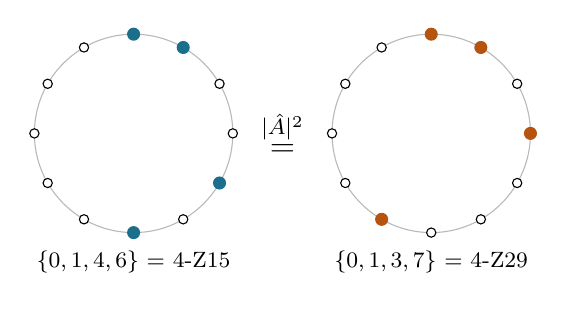
\begin{tikzpicture}[scale=0.42,every node/.style={font=\footnotesize}]
  % two clocks: the Z-pair
  \begin{scope}[shift={(0,0)}]
    \draw[gray!55] (0,0) circle (3);
    \foreach \k in {0,...,11}{
      \pgfmathtruncatemacro{\ina}{(\k==0||\k==1||\k==4||\k==6)?1:0}
      \ifnum\ina=1 \filldraw[ctA] ({90-30*\k}:3) circle (0.18);
      \else \draw[fill=white] ({90-30*\k}:3) circle (0.14); \fi}
    \node at (0,-3.9) {$\{0,1,4,6\}$ = 4-Z15};
  \end{scope}
  \begin{scope}[shift={(9,0)}]
    \draw[gray!55] (0,0) circle (3);
    \foreach \k in {0,...,11}{
      \pgfmathtruncatemacro{\inb}{(\k==0||\k==1||\k==3||\k==7)?1:0}
      \ifnum\inb=1 \filldraw[ctB] ({90-30*\k}:3) circle (0.18);
      \else \draw[fill=white] ({90-30*\k}:3) circle (0.14); \fi}
    \node at (0,-3.9) {$\{0,1,3,7\}$ = 4-Z29};
  \end{scope}
  \node at (4.5,0) {\large $\overset{|\Ahat|^2}{=}$};
\end{tikzpicture}
\caption{The $Z$-related (homometric) pair $\{0,1,4,6\}$ and $\{0,1,3,7\}$: identical power
spectrum $|\Ahat|^2=[16,2,4,2,4,2,4,2,4,2,4,2]$ and interval vector, yet not related by any
transposition or inversion. The interval vector --- a function of $|\Ahat|^2$ alone --- cannot
tell them apart; only the phase of $\Ahat$ can.}
\label{fig:p1-zpair}
\end{figure}

\subsection{The sum vector: a first glimpse of phase}\label{sec:p1-sum}

\question{P\textsubscript{4}. Can any invariant see \emph{some} of the phase the interval vector
misses?}

Where the interval vector counts tones held under transposition (the difference pairing $a-b$,
governed by $|\Ahat|^2$), the \emph{sum / index vector} counts tones held under inversion
$I_j:x\mapsto j-x$ (the sum pairing $a+b$): $\#(A\cap I_jA)=\mathrm{sumcorr}(A,j)$
(\lean{commonTonesInv\_eq\_sumcorr}), and this is the inverse DFT of the squared \emph{coefficient}
$\Ahat^2$, not the squared magnitude---so it retains phase (\lean{sumcorr\_eq\_invDFT}). It already
splits the homometric pair: about the axis $j=0$, $\{0,1,4,6\}$\,\audio{inversion_4z15.wav} holds
two tones and $\{0,1,3,7\}$\,\audio{inversion_4z29.wav} holds one
(\lean{sumVector\_distinguishes\_homometric}, by \lean{decide}). The phase the interval vector
cannot see, an inversional count can---partly.

\subsection{The phase-taxonomy capstone}\label{sec:p1-capstone}

\question{P\textsubscript{5}. What would it take to see \emph{all} of the phase?}

The full transform. $\Ahat$ is a complete invariant: $\Ahat_A=\Ahat_B\Rightarrow A=B$
(\lean{Ahat\_injective}), with biconditional \lean{Ahat\_eq\_iff}---the proof is short and
classical, since \lean{ZMod.dft} is a \lean{LinearEquiv} hence injective and the indicator recovers
membership (\lean{ind\_injective}). Passing to a set \emph{class} quotients out exactly two phase
operations: a transposition is a frequency-linear phase ramp on $\Ahat$ (\lean{tpose\_iff\_Ahat\_ramp})
and an inversion a conjugation-plus-ramp (\lean{inv\_iff\_Ahat\_conj\_ramp}), so $B$ lies in the
$T/I$ orbit of $A$ iff $\Ahat_B$ equals $\Ahat_A$ up to a ramp or up to conjugation-and-ramp
(\lean{setClass\_iff\_Ahat\_mod\_phase}). The pillar therefore closes as a ladder with two
machine-checked boundaries certified side by side: the magnitude-only floor $|\Ahat|^2$, where
homometry collapses distinct chords (P\textsubscript{3}), and the complete invariant $\Ahat$, where
nothing is lost (P\textsubscript{5}). The phase is exactly the data that completes the interval
vector to a total invariant; we return to what this says back to Pillar~2's self-duality in
Section~\ref{sec:p2-sixthirty}.

\begin{figure}[ht]
\centering
\resizebox{0.82\textwidth}{!}{%
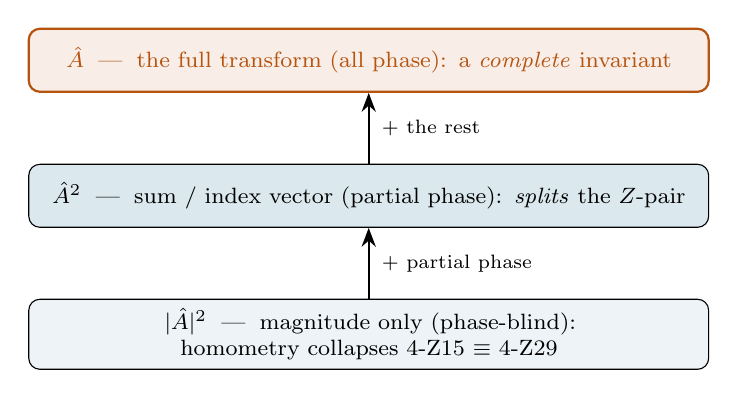
\begin{tikzpicture}[every node/.style={font=\footnotesize},>={Stealth[length=2.4mm]}]
  \node[draw,rounded corners,fill=ctA!8,text width=8.4cm,align=center,minimum height=8mm] (l1)
    {$|\Ahat|^2$ \;---\; magnitude only (phase-blind): homometry collapses $4$-Z15 $\equiv$ $4$-Z29};
  \node[draw,rounded corners,fill=ctA!16,text width=8.4cm,align=center,minimum height=8mm,above=9mm of l1] (l2)
    {$\Ahat^2$ \;---\; sum / index vector (partial phase): \emph{splits} the $Z$-pair};
  \node[draw,rounded corners,ctB,thick,fill=ctB!10,text width=8.4cm,align=center,minimum height=8mm,above=9mm of l2] (l3)
    {$\Ahat$ \;---\; the full transform (all phase): a \emph{complete} invariant};
  \draw[->,thick] (l1) -- (l2) node[midway,right=1pt,font=\scriptsize]{$+$ partial phase};
  \draw[->,thick] (l2) -- (l3) node[midway,right=1pt,font=\scriptsize]{$+$ the rest};
\end{tikzpicture}}
\caption{The taxonomy as a ladder of increasing information. The bottom rung, the power spectrum
$|\Ahat|^2$, is phase-blind, and homometry collapses the $4$-Z15 / $4$-Z29 pair onto it
(\lean{homometric\_iff\_normSq\_dft\_eq}); the squared coefficient $\Ahat^2$ restores enough phase to split
the pair (\lean{sumVector\_distinguishes\_homometric}); the full transform $\Ahat$ is a complete invariant
(\lean{Ahat\_injective}). The two boundaries --- magnitude-blind and complete --- are certified side by side.}
\label{fig:p1-ladder}
\end{figure}

\begin{table}[ht]
\centering\scriptsize\setlength{\tabcolsep}{4pt}
\rowcolors{2}{ctA!7}{white}
\begin{tabular}{@{}p{0.35\textwidth} p{0.57\textwidth}@{}}
\toprule
\rowcolor{ctA!22}
\textbf{Theorem} & \textbf{Statement}\\
\midrule
\lean{Ahat\_zero}, \lean{Ahat\_tpose}, \lean{Ahat\_compl} & $\Ahat(0)=|A|$; transposition $=$ phase ramp; complement $=$ negation off DC.\\
\lean{IVraw\_tpose}, \lean{IVraw\_invert} & interval vector invariant under $T$ and $I$.\\
\lean{autocorr\_eq\_invDFT} & Wiener--Khinchin: $\mathrm{autocorr}=\Fi(|\Ahat|^2)$.\\
\lean{IVraw\_eq\_invDFT\_power} & \textbf{keystone}: interval vector $=\Fi(|\Ahat|^2)$ regraded by class.\\
\lean{hexachord\_powerSpec\_eq}, \lean{hexachord\_IVraw\_eq} & Babbitt: hexachord and complement share $|\Ahat|^2$, hence interval content.\\
\lean{commonTones\_eq\_invDFT}, \lean{IVraw\_tritone} & common tones $=\Fi(|\Ahat|^2)$; tritone factor (singleton fibre).\\
\lean{IsDeep\_iff\_commonTones\_nodup} & deep $\iff$ distinct transposition common-tone counts.\\
\lean{rop\_iff\_autocorr\_zero}, \lean{rop\_card\_le} & rhythmic oddity $\iff \mathrm{autocorr}(\cdot,6)=0$; forces $|A|\le6$.\\
\lean{homometric\_iff\_normSq\_dft\_eq} & homometry $\iff$ equal $|\Ahat|^2$ (the discrete phase problem).\\
\lean{allIntervalTetrachords\_homometric} & $\{0,1,4,6\}\sim\{0,1,3,7\}$ (4-Z15 / 4-Z29), the $Z$-witness.\\
\lean{sumcorr\_eq\_invDFT}, \lean{sumVector\_distinguishes\_homometric} & sum vector $=\Fi(\Ahat^2)$ (partial phase); splits the $Z$-pair.\\
\lean{Ahat\_injective}, \lean{Ahat\_eq\_iff} & the full $\Ahat$ is a complete invariant.\\
\lean{setClass\_iff\_Ahat\_mod\_phase} & set class $=\Ahat$ up to a phase ramp / conjugation-and-ramp.\\
\bottomrule
\end{tabular}
\caption{Pillar~1 in \lean{Fourier.lean} / \lean{IntervalVector.lean}: the invariants on the
ladder of phase, sorry-free with axiom audit $[\mathrm{propext},\mathrm{Classical.choice},
\mathrm{Quot.sound}]$ (the \lean{decide} witnesses choice-free). Novelty is adjudicated in
Section~\ref{sec:novelty}.}
\label{tab:p1}
\end{table}
     % \S\ref{sec:pillar1}
% pillar2_duality.tex -- Pillar 2 body of corpus_paper.tex, in the HOUSE LINE.
% No preamble: relies on the master's macros. Honesty (the 6-30 = ours; CFS = first-formaliz.)
% lives in the master's Novelty section (Sec. \ref{sec:novelty}) -- NO inline tags here.
% Source of exposition: Note #1 (sixthirty_note.tex); content audited against NeoRiemannian.lean
% and SixThirty.lean.

\section{Pillar 2: Transformational duality}\label{sec:pillar2}

\question{P\textsubscript{0}. A group that acts simply transitively has a \emph{dual} that mirrors
it. What does that dual do for a triad---and what happens to it for a \emph{symmetric} chord?}

The neo-Riemannian tradition reads chords not by their notes but by the group of operations
relating them, and pairs each transformation group with a dual: two subgroups of
$\mathrm{Sym}(\Omega)$ are \emph{dual} in Lewin's sense (\cite{Lewin}, p.~157) when each is the
centralizer of the other and both act simply transitively. This pillar machine-checks that duality
for the $24$ triads, then follows it into the one place it does something new---a symmetric chord,
where the tritone is the center of the group.

\subsection{The $T/I$ action on triads and the $PLR$ group}\label{sec:p2-ti}

A \emph{triad} is a pair $(\mathrm{root},\mathrm{quality})\in\Ztwelve\times\mathrm{Bool}$ (major
$\{r,r{+}4,r{+}7\}$ or minor $\{r,r{+}3,r{+}7\}$); there are $24$. The $T/I$ group is Mathlib's
\lean{DihedralGroup}\,$12$, acting on triads simply transitively---the left regular representation
(\lean{card\_TIgrp}\,$=24$, with \lean{MulAction}, \lean{IsPretransitive} and \lean{FaithfulSMul}
instances). The neo-Riemannian operations $P,L,R$ are the three involutions that exchange a triad
with the one sharing two common tones (\lean{Pf},\lean{Lf},\lean{Rf}); each commutes with every
$T/I$ operation (\lean{Pf\_comm}, \lean{Lf\_comm}, \lean{Rf\_comm}), and each is a minimal
voice-leading move: $P$ and $L$ shift one voice by a semitone (\lean{P\_size\_one},
\lean{L\_size\_one}), $R$ by a whole tone (\lean{R\_size\_two}), each holding the other
two tones fixed (\lean{P\_holds\_two}, \lean{L\_holds\_two}, \lean{R\_holds\_two})---this is the
parsimony Cohn~\cite{Cohn} built the Tonnetz on.

\subsection{$PLR$ is the centralizer of $T/I$ (Crans--Fiore--Satyendra)}\label{sec:p2-cfs}

\question{P\textsubscript{1}. The triad is asymmetric, so its orbit has $24$ forms. Is the
$PLR$ group really the \emph{whole} dual---and why?}

The duality is the regular case of the classical centralizer theorem: the centralizer of a regular
permutation group is its opposite regular representation (Dixon--Mortimer~\cite{DM} \S4.2,
Cameron~\cite{Cam}). Its engine is a single lemma---an element of the centralizer that fixes one
point is the identity (\lean{centralizing\_fixedPoint\_eq\_one})---which was \emph{absent} from
Mathlib and which we supply. From it: $\langle P,L,R\rangle$ lies in the centralizer
(\lean{PLR\_le\_centralizer}), the centralizer has at most $24$ elements and $PLR$ has exactly $24$
(\lean{card\_PLRgrp}), and the two coincide,
\[
  \mathrm{centralizer}(T/I)=\langle P,L,R\rangle\qquad(\lean{centralizer\_eq\_PLR}),
\]
the Crans--Fiore--Satyendra duality~\cite{CFS}.

\subsection{The 6-30 tritone-centered self-duality}\label{sec:p2-sixthirty}

\question{P\textsubscript{2}. What happens to the dual when the object is a \emph{symmetric} chord,
whose orbit is smaller than $24$?}

A symmetric class has a nontrivial $T/I$-stabilizer, so its orbit is smaller and the action is no
longer free; a reduced simply-transitive dual survives exactly when the stabilizer is \emph{normal}
in $\Dgrp{12}$, and among order-$2$ symmetries that singles out the center $\{T_0,T_6\}$---the
tritone. The unique nontrivial set class in $\Ztwelve$ with exactly that symmetry is Forte
\textbf{6-30}$=\{0,1,3,6,7,9\}$, the set class of Stravinsky's Petrushka chord
(Figure~\ref{fig:p2-clock}): exhaustive enumeration over the $222$ nontrivial pitch-class set
classes of $\Ztwelve$ confirms there is no other class whose $T/I$-stabilizer is precisely
$\{T_0,T_6\}$ (a finite check, reported in Note~\#1~\cite{Note1}). It is the union of the three
central pairs $\{0,6\},\{1,7\},\{3,9\}$,
so it is fixed by the tritone $T_6$ (\lean{T6\_invariant})\,\audio{t6_symmetry.wav} and has no
inversional symmetry (\lean{not\_inversionally\_symmetric}). Its $T/I$-orbit therefore collapses to
$12$ (\lean{card\_O}); the tritone lands in the kernel of the action on the orbit
(\lean{Ker\_eq}\,$=\{1,r_6\}$); and the dual---the centralizer of the reduced action---has order
$12$ (\lean{card\_Cgrp}, built as the opposite regular representation), is transitive hence regular
(\lean{Cgrp\_transitive}), and carries the dihedral fingerprint (\lean{dihedral\_fingerprint}: an
order-$6$ generator $s$, an involution $t\neq1$ with $tst=s^{-1}$ and $st\neq ts$), pinning it as
dihedral of order $12$. So the twelve forms of the Petrushka chord form a single navigable harmonic
space\,\audio{orbit_12.wav}, the symmetric-chord analogue of the $P/L/R$ network for triads---the
tritone Stravinsky reached for by ear \emph{is} the central symmetry $T_6$, and that center is
exactly what endows 6-30 with its order-12 self-duality.

\begin{figure}[ht]
\centering
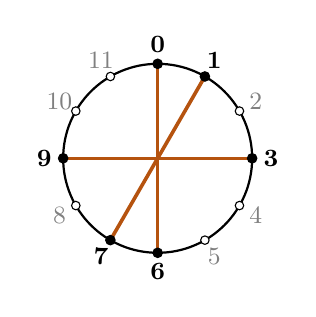
\begin{tikzpicture}[scale=1.2,every node/.style={font=\small}]
  \draw[thick] (0,0) circle (1);
  \foreach \a/\b in {0/6,1/7,3/9}{
    \draw[ctB,line width=1.3pt] ({90-30*\a}:1) -- ({90-30*\b}:1);}
  \foreach \k in {0,...,11}{
    \pgfmathtruncatemacro{\ina}{(\k==0||\k==1||\k==3||\k==6||\k==7||\k==9)?1:0}
    \ifnum\ina=1 \filldraw[black] ({90-30*\k}:1) circle (0.05);
      \node at ({90-30*\k}:1.2) {\textbf{\k}};
    \else \draw[fill=white] ({90-30*\k}:1) circle (0.045);
      \node[gray] at ({90-30*\k}:1.2) {\k}; \fi}
\end{tikzpicture}
\caption{\textbf{6-30}$=\{0,1,3,6,7,9\}$ on the pitch-class clock: the union of the three central
pairs $\{0,6\},\{1,7\},\{3,9\}$ (heavy tritone diameters), hence fixed by $T_6$ (a $180^\circ$
rotation) and, with no inversional symmetry, stabilized by exactly $\{T_0,T_6\}$. That central
stabilizer is what reduces the orbit to $12$ and makes the dual dihedral of order $12$.}
\label{fig:p2-clock}
\end{figure}

\begin{figure}[ht]
\centering
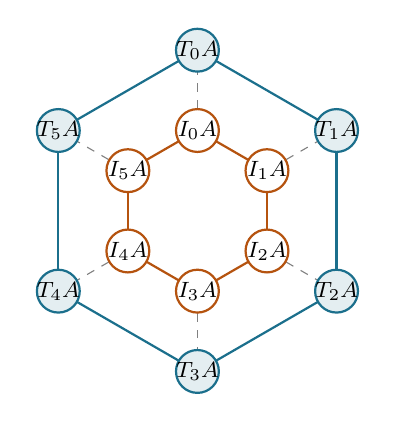
\begin{tikzpicture}[scale=0.85,every node/.style={font=\footnotesize},>={Stealth[length=2mm]}]
  \foreach \k in {0,...,5}{
    \coordinate (O\k) at ({90-60*\k}:2.4);
    \coordinate (I\k) at ({90-60*\k}:1.2);}
  \foreach \k in {0,...,5}{
    \pgfmathtruncatemacro{\nextk}{mod(\k+1,6)}
    \draw[ctA,->,thick] (O\k) -- (O\nextk);
    \draw[ctB,->,thick] (I\nextk) -- (I\k);
    \draw[gray,dashed] (O\k) -- (I\k);}
  \foreach \k in {0,...,5}{
    \filldraw[fill=ctA!12,draw=ctA,thick] (O\k) circle (0.32) node[black]{$T_{\k}A$};
    \filldraw[fill=white,draw=ctB,thick] (I\k) circle (0.32) node[black]{$I_{\k}A$};}
\end{tikzpicture}
\caption{The order-$12$ dual group $\Dgrp{6}$ acting simply transitively on the $12$ forms of $6$-$30$ ---
its Cayley graph, the symmetric-chord analogue of the $P/L/R$ network for triads. Outer nodes are the six
transposition forms $T_kA$ (with $T_kA=T_{k+6}A$ identified), inner nodes the six inversion forms $I_kA$;
the solid arrows are an order-$6$ rotation generator (orientation reverses on the inner coset, as in any
dihedral Cayley graph), the dashed edges an order-$2$ reflection generator. Any form of the Petrushka chord
reaches any other by a unique dual move (\lean{Cgrp\_transitive}), so the twelve forms become a single
navigable harmonic space.}
\label{fig:p2-cayley}
\end{figure}

\subsection{The duality thread across pillars}\label{sec:p2-thread}

The shape here---a simply transitive action and its self-centralizing mirror---returns in Pillar~3.
There, regular temperament theory pairs the lattice of vals with the lattice of commas over
$\mathbb{Z}$-modules: the same flavour of duality, a generated structure and its annihilator. This
is a structural parallel, not a theorem unifying the two (Section~\ref{sec:novelty}). And the
self-duality of a symmetric chord is, in Fourier terms, a phase fact $|\Ahat|$ cannot see
(\S\ref{sec:p1-capstone})---$T_6$-symmetry is even-frequency support, a magnitude statement, but
which symmetric chords are self-dual needs the phase, the same blindness as the $Z$-relation.

\begin{table}[ht]
\centering\scriptsize\setlength{\tabcolsep}{4pt}
\rowcolors{2}{ctB!7}{white}
\begin{tabular}{@{}p{0.37\textwidth} p{0.55\textwidth}@{}}
\toprule
\rowcolor{ctB!22}
\textbf{Theorem} & \textbf{Statement}\\
\midrule
\multicolumn{2}{@{}l}{\emph{the duality engine, \lean{NeoRiemannian.lean}}}\\
\lean{card\_TIgrp} & $T/I$ acts on the $24$ triads as the regular rep of $\Dgrp{12}$.\\
\lean{Pf\_comm}, \lean{Lf\_comm}, \lean{Rf\_comm} & $P,L,R$ each commute with the $T/I$ action.\\
\lean{P\_size\_one}, \lean{L\_size\_one}, \lean{R\_size\_two} & minimal voice-leading sizes of $P,L,R$.\\
\lean{centralizing\_fixedPoint\_eq\_one} & Wielandt regular case (centralizer is semiregular) --- a Mathlib gap.\\
\lean{centralizer\_eq\_PLR} & $\mathrm{centralizer}(T/I)=\langle P,L,R\rangle$ (CFS duality); \lean{card\_PLRgrp}$=24$.\\
\multicolumn{2}{@{}l}{\emph{the 6-30 self-duality, \lean{SixThirty.lean}}}\\
\lean{T6\_invariant}, \lean{not\_inversionally\_symmetric} & $A=\{0,1,3,6,7,9\}$ fixed by $T_6$, no inversion symmetry.\\
\lean{card\_O}, \lean{Ker\_eq} & orbit $12$; kernel of the action $=\{T_0,T_6\}=Z(\Dgrp{12})$.\\
\lean{card\_Cgrp}, \lean{Cgrp\_transitive} & dual (centralizer on the orbit) order $12$, regular.\\
\lean{dihedral\_fingerprint} & order $12$; $s^6{=}1$, $t^2{=}1{\neq}t$, $tst{=}s^{-1}$, $st{\neq}ts$ (dihedral).\\
\bottomrule
\end{tabular}
\caption{Pillar~2 in \lean{NeoRiemannian.lean} / \lean{SixThirty.lean}, sorry-free with axiom audit
$[\mathrm{propext},\mathrm{Classical.choice},\mathrm{Quot.sound}]$. The 6-30 dual is the one place
the paper goes beyond formalization; its scope and the relation to the Fiore lineage are stated in
Section~\ref{sec:novelty}.}
\label{tab:p2}
\end{table}
     % \S\ref{sec:pillar2}
% pillar3_scales_tuning.tex -- Pillar 3 body of corpus_paper.tex, in the HOUSE LINE.
% No preamble: relies on the master's macros. Honesty (all first-formaliz.; the step-gap-vs-
% all-pairs framing point) lives in the master's Novelty section (Sec. \ref{sec:novelty}).
% Content audited against DiatonicScale.lean, MaximalEvenness.lean, AllPairsEvenness.lean,
% Temperament.lean, CircleOfFifths.lean.
% TODO(audio): generate scale/tuning sonifications (diatonic, circle of fifths, comma drift)
%   for the public repo and add \audio links; for now one relevant link (modes_messiaen).

\section{Pillar 3: scales and tuning}\label{sec:pillar3}

\question{P\textsubscript{0}. Why is the diatonic scale special---and is its specialness one fact,
or several that happen to coincide?}

Four regularity conditions on a scale---being generated by a single interval, being well-formed,
having Myhill's property, being maximally even---pick out the diatonic, and the last reconnects to
the autocorrelation of Pillar~1. This pillar machine-checks each, names the instance where only an
instance is proven, and ends at the tuning lattices where the duality thread of Pillar~2 returns.

\subsection{Generated and well-formed scales}\label{sec:p3-genwf}

Stacking $k$ perfect fifths from a starting pitch and reducing mod $12$ (\lean{stack}) generates
the diatonic at $k=7$ (\lean{diatonic\_generated\_by\_fifth}) and the pentatonic at $k=5$
(\lean{pentatonic\_generated\_by\_fifth}). A scale is \emph{well-formed} when it has exactly two
step sizes (\lean{IsWellFormed}). The diatonic is well-formed, with steps $\{1,2\}$ semitones
(\lean{diatonic\_isWellFormed}, \lean{diatonic\_stepSizes}), and so is the pentatonic, with steps
$\{2,3\}$ (\lean{pentatonic\_isWellFormed}); stacking too far breaks it --- six fifths give three
step sizes (\lean{sixFifths\_not\_wellFormed}). That a generated scale has at most \emph{three} step sizes is
the three-gap (Steinhaus) theorem, which we verify in $\Ztwelve$ (\lean{threeGap\_chromatic};
Sós~\cite{Steinhaus}). Carey--Clampitt's well-formedness theory~\cite{CareyClampitt} is the frame.

\subsection{Myhill's property}\label{sec:p3-myhill}

\question{P\textsubscript{1}. Well-formedness counts step sizes. Myhill's property counts something
finer---and it separates the diatonic from its even cousin.}

A scale has Myhill's property when every nonzero generic interval (second, third, \dots) comes in
exactly two specific sizes (\lean{HasMyhill}). The diatonic does (\lean{diatonic\_hasMyhill}); the
whole-tone scale does \emph{not} (\lean{wholeTone\_not\_hasMyhill}), its single whole-step
collapsing the variety. By Carey--Clampitt, Myhill is equivalent to non-degenerate
well-formedness; we formalize the diatonic instance and the whole-tone counterexample, and note the
general equivalence (which needs Christoffel/three-gap word machinery, thin in Mathlib) as not yet
formalized.

\subsection{Maximal evenness}\label{sec:p3-me}

\question{P\textsubscript{2}. ``Spread $k$ notes as evenly as possible'': which energy makes that
precise, and does it actually single out the diatonic?}

Maximal evenness (Clough--Douthett~\cite{CloughDouthett}) is the deepest of the four conditions, and
we formalize it in three layers, explicit about which energy does the work\,\audio{modes_messiaen.wav}.
\emph{(i) The predicate.} A scale is maximally even when each generic interval takes at most two
specific sizes and those are consecutive integers (\lean{IsMaxEven}); the diatonic and the
whole-tone scale both qualify (\lean{diatonic\_isMaxEven}, \lean{wholeTone\_isMaxEven}), so maximal
evenness strictly contains Myhill (the whole-tone scale is maximally even but, by
\S\ref{sec:p3-myhill}, not Myhill). \emph{(ii) The step-gap energy.} For a strictly convex potential
$V$, the energy $\sum_i V(\text{gap}_i)$ over the circular step gaps is minimized exactly at the
\emph{balanced} configurations, $\max-\min\le1$ (\lean{isMinimizer\_iff\_balanced}), via a
strict-convexity swap lemma and a well-founded descent. This characterizes the balanced step
multiset---a \emph{necessary} condition for maximal evenness, but not sufficient, and we say so in
Section~\ref{sec:novelty}. \emph{(iii) The all-pairs energy.} The energy that uniquely selects the
diatonic is the Douthett--Krantz all-pairs Hamiltonian $E(V,A)=\sum_{a<b}V(\mathrm{cdist}(a,b))$
over all pairwise distances. For every decreasing-convex $V$ the diatonic minimizes it, and for
every strictly such $V$ it is the \emph{unique} minimizer up to transposition and inversion
(\lean{diatonic\_ground\_state}, \lean{diatonic\_unique})---one statement holding simultaneously for
all admissible potentials, the $V$-independence. The engine is a double summation-by-parts identity
(\lean{abel\_bridge}): two $k$-subsets have equal interval-vector totals $\binom{k}{2}$, so their
difference sums to zero and the energy gap collapses to a sum of double-cumulative sums against the
convexity of $V$. The same theorem holds for the other maximally even
cardinalities in $\Ztwelve$ --- pentatonic ($k=5$), whole-tone ($k=6$), octatonic ($k=8$), joining
the diatonic ($k=7$) --- (\lean{pentatonic\_unique}, \lean{wholetone\_unique},
\lean{octatonic\_unique}), via a cardinality-independent core. (Equivalently the diatonic uniquely maximizes $|\Ahat(5)|$,
Quinn~\cite{Quinn}---Pillar~1's autocorrelation thread, returning.)

\subsection{Regular temperament theory: vals and comma lattices}\label{sec:p3-rtt}

\question{P\textsubscript{3}. Twelve fifths nearly close the octave; the gap is the Pythagorean
comma. What is the algebra of ``nearly''?}

Model a pitch by its exponents in the prime generators: a val is a $\mathbb{Z}$-linear map sending
generators to step counts (\lean{v12}, \lean{v5}, \lean{v7}). Twelve fifths minus seven octaves is
the Pythagorean comma $\mathrm{pc}$ (\lean{closure\_defect\_eq\_pc}); $12$-tone equal temperament is
exactly the val that annihilates it, and the comma generates the whole rank-$1$ kernel,
$\ker v_{12}=\mathbb{Z}\cdot\mathrm{pc}$ (\lean{ker\_v12\_eq\_span\_pc}), with only the
$12$-val killing it (\lean{only\_twelve\_tempers\_pc}). In the $5$-limit the syntonic comma enters:
$12$-ET tempers it (\lean{v12\_5\_tempers\_syntonic}), four fifths equal a major third up to that
comma (\lean{meantone\_defect\_eq\_syntonic})---so $12$-ET is a meantone---and the comma kernel is
rank $2$, spanned by the syntonic and Pythagorean commas (\lean{ker\_v12\_5\_eq\_span}). Reducing the
fifth mod $12$ closes the circle of fifths onto all twelve pitch classes
(\lean{circle\_of\_fifths\_complete}, Figure~\ref{fig:p3-fifths}), and four fifths reduce to the
major third (\lean{four\_fifths\_eq\_major\_third}). The val--comma pairing---a generated lattice and
its annihilator---is the $\mathbb{Z}$-module echo of Pillar~2's centralizer duality, the rhyme of
\S\ref{sec:p2-thread}.

\begin{figure}[ht]
\centering
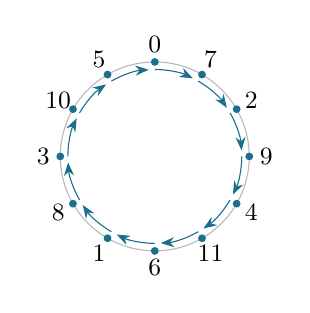
\begin{tikzpicture}[scale=1.2,every node/.style={font=\small}]
  \draw[gray!55] (0,0) circle (1);
  \foreach \i in {0,...,11}{
    \pgfmathtruncatemacro{\pc}{mod(7*\i,12)}
    \coordinate (n\i) at ({90-30*\i}:1);
    \filldraw[ctA] (n\i) circle (0.035);
    \node at ({90-30*\i}:1.18) {\pc};}
  \foreach \i in {0,...,11}{
    \pgfmathtruncatemacro{\j}{mod(\i+1,12)}
    \draw[ctA,->,>=Stealth,thin] ({90-30*\i}:0.92) arc ({90-30*\i}:{90-30*\i-26}:0.92);}
\end{tikzpicture}
\caption{The circle of fifths: stepping by the reduced fifth ($7$ semitones) visits all twelve
pitch classes (\lean{circle\_of\_fifths\_complete}); the node labels are the pitch classes reached
in fifth-order. Closure is the rank-$1$ comma kernel of \lean{ker\_v12\_eq\_span\_pc}.}
\label{fig:p3-fifths}
\end{figure}

\begin{table}[ht]
\centering\scriptsize\setlength{\tabcolsep}{4pt}
\rowcolors{2}{ctA!7}{white}
\begin{tabular}{@{}p{0.40\textwidth} p{0.52\textwidth}@{}}
\toprule
\rowcolor{ctA!22}
\textbf{Theorem} & \textbf{Statement}\\
\midrule
\lean{diatonic\_generated\_by\_fifth}, \lean{pentatonic\_generated\_by\_fifth} & diatonic / pentatonic generated by stacked fifths.\\
\lean{diatonic\_isWellFormed}, \lean{sixFifths\_not\_wellFormed} & well-formed $=$ two step sizes; the boundary.\\
\lean{threeGap\_chromatic} & three-gap / Steinhaus theorem in $\Ztwelve$.\\
\lean{diatonic\_hasMyhill}, \lean{wholeTone\_not\_hasMyhill} & Myhill's property: diatonic yes, whole-tone no.\\
\lean{diatonic\_isMaxEven}, \lean{wholeTone\_isMaxEven} & maximal evenness (predicate); ME $\supsetneq$ MP.\\
\lean{isMinimizer\_iff\_balanced} & step-gap energy minimizer $\iff$ balanced multiset (necessary, not sufficient).\\
\lean{diatonic\_ground\_state}, \lean{diatonic\_unique} & all-pairs energy: diatonic the unique minimizer up to $T/I$, $\forall$ admissible $V$.\\
\lean{pentatonic\_unique}, \lean{wholetone\_unique}, \lean{octatonic\_unique} & same, at $k\in\{5,6,8\}$, via \lean{abel\_bridge}.\\
\lean{closure\_defect\_eq\_pc}, \lean{ker\_v12\_eq\_span\_pc} & Pythagorean comma $=$ closure defect; rank-$1$ kernel.\\
\lean{meantone\_defect\_eq\_syntonic}, \lean{ker\_v12\_5\_eq\_span} & syntonic comma / meantone; rank-$2$ $5$-limit kernel.\\
\lean{circle\_of\_fifths\_complete}, \lean{four\_fifths\_eq\_major\_third} & twelve fifths generate $\Ztwelve$; $4$ fifths $=$ major third.\\
\bottomrule
\end{tabular}
\caption{Pillar~3 in \lean{DiatonicScale.lean}, \lean{MaximalEvenness.lean},
\lean{AllPairsEvenness.lean}, \lean{Temperament.lean}, \lean{CircleOfFifths.lean}, sorry-free; axiom
audit $[\mathrm{propext},\mathrm{Classical.choice},\mathrm{Quot.sound}]$, except the finite
all-pairs censuses, which additionally carry $\mathrm{Lean.ofReduceBool}$ (\lean{native\_decide}),
flagged in Section~\ref{sec:novelty}.}
\label{tab:p3}
\end{table}
 % \S\ref{sec:pillar3}

\section{Novelty, scope, and what this work does not claim}\label{sec:novelty}

\question{What here is new mathematics, what is a first formalization of known mathematics, and
what is merely organization? We answer in one place, ruthlessly, so the framing cannot drift.}

\paragraph{Contribution, stated plainly.} This is a formalization paper. With the two exceptions
below, every result is a machine-checked proof of a published theorem --- to our knowledge a first
formalization --- cited to its source
in its pillar and collected in Table~\ref{tab:ledger}. The library is sorry-free; the axiom
audit is $[\mathrm{propext},\,\mathrm{Classical.choice},\,\mathrm{Quot.sound}]$ throughout, save
the finite maximal-evenness censuses, which additionally carry $\mathrm{Lean.ofReduceBool}$ from
\lean{native\_decide}---flagged here as in the body, with the analytic engine behind them
(a double summation-by-parts identity) kept axiom-clean.

\paragraph{What is genuinely ours (1): the 6-30 self-duality.} The one place where we believe we
go beyond formalization is the tritone-centered order-$12$ self-duality of the Petrushka set
class $6$-$30=\{0,1,3,6,7,9\}$ (\S\ref{sec:p2-sixthirty}). It is not inversionally symmetric yet
is fixed by the tritone $T_6$; its $T/I$-orbit therefore collapses to $12$, the tritone lands in
the kernel of the action, and the centralizer of the reduced action is dihedral of order $12$.
We are unaware of a previous explicit characterization of this dual, or of a machine-checked
contextual dual of a symmetric chord. We state it \emph{measuredly}, as in Note~\#1~\cite{Note1}: it is \emph{complementary} to the Fiore
lineage rather than something they missed. Fiore--Satyendra~\cite{FS} and
Fiore--Noll~\cite{FN11,FN25} each sidestep the reduced-orbit tritone-central regime;
\cite{FN11} even tabulates the same set class as a point and studies its order-$2$ cover, never
forming the order-$12$ dual of the hexachord-as-a-point. Berry--Fiore~\cite{BF} prove the same
centralizer duality for hexatonic cycles---a different object (augmented stabilizer, dual $S_3$
of order $6$). The one residual collision risk, Peck's generalized commuting groups~\cite{Peck},
is hedged, not dismissed; the published octatonic commuting groups in this lineage are order
$8$, not $12$. What we claim is the explicit characterization and its machine-checked dual, not
priority over the general theory.

\paragraph{What is genuinely ours (2): the unified phase taxonomy.} Every ingredient of the phase
taxonomy is classical (Patterson, Lewin, Babbitt, Amiot). What we believe is unstated \emph{as a
single statement} is the unification: pinning each invariant to its exact slice of $\Ahat$ and
certifying both boundaries of the ladder---the magnitude-blind collapse (homometry) and the
complete-invariant capstone---side by side, with one axiom audit (\S\ref{sec:p1-capstone}). This
is organization, not new mathematics; we claim priority over none of the underlying results.

\paragraph{A smaller framing point.} In the scale theory we make explicit that the convex-energy
characterization of maximal evenness splits into a degenerate step-gap form and a
diatonic-selecting all-pairs form (\S\ref{sec:p3-me}); this is a clarification of which object
does the work, not a theorem.

\paragraph{Prior proof-assistant work.} The only prior Lean music formalization we are aware of
(Prismriver~\cite{Prismriver}) addresses the $T/I$ action; the three layers here---the DFT /
interval-vector invariants, the neo-Riemannian duality, and scale and tuning theory---are, to
our knowledge, first formalizations. One reusable group-theory lemma, the regular case of
Wielandt's centralizer theorem (\lean{centralizing\_fixedPoint\_eq\_one}), was absent from
Mathlib and is supplied here.

\begin{table}[H]
\centering\small
\setlength{\tabcolsep}{5pt}
\rowcolors{2}{ctA!7}{white}
\begin{tabular}{@{}p{0.40\textwidth} p{0.34\textwidth} c@{}}
\toprule
\rowcolor{ctA!22}
\textbf{Result} & \textbf{Classical source} & \textbf{Status}\\
\midrule
\multicolumn{3}{@{}l}{\emph{Pillar 1 --- Fourier invariants}}\\
Interval vector $=\Fi|\Ahat|^2$; common tones & Amiot~\cite{Amiot}; Lewin~\cite{Lewin},Rahn~\cite{Rahn} & first-formaliz.\\
Babbitt's hexachord theorem & Babbitt; Lewin~\cite{Lewin1960} & first-formaliz.\\
Deep scales; rhythmic oddity & Gamer/Browne~\cite{Browne}; Chemillier--Truchet~\cite{ChemillierTruchet} & first-formaliz.\\
Homometry $=$ phase problem & Patterson~\cite{Patterson}; Forte~\cite{Forte} & first-formaliz.\\
Unified phase taxonomy (one statement) & --- (this work) & \textbf{ours: organization}\\
\multicolumn{3}{@{}l}{\emph{Pillar 2 --- Transformational duality}}\\
$T/I$ regular rep; $PLR$ voice-leading & Lewin~\cite{Lewin}; Cohn~\cite{Cohn} & first-formaliz.\\
Wielandt regular-case lemma & Dixon--Mortimer~\cite{DM} & first-formaliz.$^\dagger$\\
CFS duality: $PLR=$ centralizer$(T/I)$ & Crans--Fiore--Satyendra~\cite{CFS} & first-formaliz.\\
\textbf{6-30 tritone-centered self-duality} & --- (this work) & \textbf{ours: new result}\\
\multicolumn{3}{@{}l}{\emph{Pillar 3 --- Scales and tuning}}\\
Myhill; well-formed; three-gap & Carey--Clampitt~\cite{CareyClampitt}; three-gap & first-formaliz.\\
Maximal evenness (predicate; energy) & Clough--Douthett~\cite{CloughDouthett}; Douthett--Krantz~\cite{DouthettKrantz} & first-formaliz.\\
\quad step-gap vs all-pairs distinction & --- (this work) & ours: organization\\
Comma lattices (Pythagorean, syntonic) & regular temperament theory & first-formaliz.\\
\bottomrule
\end{tabular}
\caption{The honesty ledger. Every row is a first formalization of classical mathematics, cited
to its source, except the two \textbf{ours} rows (one new result, one organization) and the
smaller framing point. $^\dagger$ The Wielandt regular-case lemma was absent from Mathlib;
supplying it is a small reusable formalization contribution beyond the music content.}
\label{tab:ledger}
\end{table}

\section{The open frontier}\label{sec:frontier}

\question{What can we state but not yet certify in the kernel---and where does each thread point
next?}

In the spirit of the wider program, we treat the boundary of what is formalized as an output,
not a gap to be hidden. Four directions stand open.

\begin{itemize}\itemsep2pt
  \item \textbf{The general-$n$ self-dual family.} The reduced-duality characterization behind
        $6$-$30$ is universe-independent; $6$-$30$ is the minimal nontrivial instance of a family
        with dual $\cong\Dgrp{n/2}$ at universe $n$ (the count is OEIS A032239). A uniform Lean
        statement, and the named isomorphism $\Dgrp{12}/Z\cong\Dgrp{6}$ (currently a Mathlib gap,
        witnessed in GAP), are open.
  \item \textbf{Maximal evenness in general $(k,n)$.} The all-pairs $V$-independent uniqueness is
        certified over $\Ztwelve$ for $k\in\{5,6,7,8\}$ by finite census; the analytic engine (the
        double summation-by-parts identity) is general, but the general-$(k,n)$ theorem needs the
        abstract majorization argument, and replacing the censuses by a kernel proof would retire
        the lone \lean{Lean.ofReduceBool} dependence.
  \item \textbf{Phase and self-duality.} $T_6$-symmetry is exactly even-frequency support of
        $\Ahat$, a magnitude fact; but self-duality needs phase information $|\Ahat|$ cannot
        see---the same blindness as the $Z$-relation. A phase-space account of self-duality, and a
        Lean theorem for set-class completeness (currently computational), are open.
  \item \textbf{From analysis to composition.} The library is an analysis engine; the maximally
        even generator, the well-formed phase diagram, and the dual-group navigation of a
        symmetric chord are constructive and point toward a synthesis program downstream.
\end{itemize}

\section*{Data and code availability}
The Lean sources, the Sage/GAP witness scripts, and the figures accompany this paper; each Lean
theorem is checkable by \lean{\#print axioms} and each script is re-runnable. The three
constituent notes are archived on Zenodo (\cite{Note1,Note2,Note3}).

\begin{thebibliography}{99}
% --- the DFT / Fourier thread ---
\bibitem{Loeffler} D. Loeffler, Mathlib \lean{ZMod.dft} (Apache-2.0) --- the discrete Fourier
  transform on \lean{ZMod N} as a \lean{LinearEquiv}.
\bibitem{Amiot} E. Amiot, \emph{Music Through Fourier Space: Discrete Fourier Transform in Music
  Theory}, Computational Music Science, Springer, 2016.
\bibitem{Patterson} A. L. Patterson, ``A Fourier Series Method for the Determination of the
  Components of Interatomic Distances in Crystals,'' \emph{Phys. Rev.} \textbf{46} (1934),
  372--376.
\bibitem{MAAA} J. Mandereau, D. Ghisi, E. Amiot, M. Andreatta, C. Agon, ``Z-relation and
  homometry in musical distributions,'' \emph{J. Math. \& Music} \textbf{5} (2011), no.~2,
  83--98.
\bibitem{Quinn} I. Quinn, ``General equal-tempered harmony,'' \emph{Perspectives of New Music}
  \textbf{44}--\textbf{45} (2006--2007).
% --- set theory / invariants ---
\bibitem{Forte} A. Forte, \emph{The Structure of Atonal Music}, Yale Univ. Press, 1973.
\bibitem{Lewin} D. Lewin, \emph{Generalized Musical Intervals and Transformations}, Yale Univ.
  Press, 1987 (repr.\ Oxford Univ. Press, 2007); GIS $=$ simply transitive action, p.~157.
\bibitem{Lewin1959} D. Lewin, ``Intervallic relations between two collections of notes,''
  \emph{J. Music Theory} \textbf{3} (1959), no.~2, 298--301.
\bibitem{Lewin1960} D. Lewin, ``Re: The intervallic content of a collection of notes\dots,''
  \emph{J. Music Theory} \textbf{4} (1960), no.~1, 98--101.
\bibitem{Rahn} J. Rahn, \emph{Basic Atonal Theory}, Longman, 1980.
\bibitem{Browne} R. Browne, ``Tonal implications of the diatonic set,'' \emph{In Theory Only}
  \textbf{5} (1981), no.~6--7, 3--21; C. Gamer, ``Some combinational resources of equal-tempered
  systems,'' \emph{J. Music Theory} \textbf{11} (1967), 32--59.
\bibitem{ChemillierTruchet} M. Chemillier, C. Truchet, ``Computing the rhythmic oddity property,''
  \emph{Inform. Process. Lett.} \textbf{86} (2003), no.~5, 255--261; G. T. Toussaint, \emph{The
  Geometry of Musical Rhythm}, CRC Press, 2013.
% --- transformational / duality ---
\bibitem{Cohn} R. Cohn, ``Neo-Riemannian operations, parsimonious trichords, and their Tonnetz
  representations,'' \emph{J. Music Theory} \textbf{41} (1997), no.~1, 1--66.
\bibitem{CFS} A. S. Crans, T. M. Fiore, R. Satyendra, ``Musical actions of dihedral groups,''
  \emph{Amer. Math. Monthly} \textbf{116} (2009), no.~6, 479--495 (arXiv:0711.1873).
\bibitem{DM} J. D. Dixon, B. Mortimer, \emph{Permutation Groups}, Springer GTM 163, 1996
  (\S4.2, Theorem 4.2A).
\bibitem{Cam} P. J. Cameron, \emph{Permutation Groups}, LMS Student Texts 45, CUP, 1999.
\bibitem{BF} C. Berry, T. M. Fiore, ``Hexatonic systems and dual groups in mathematical music
  theory,'' \emph{Involve} \textbf{11} (2018), no.~2, 253--270 (arXiv:1602.02577).
\bibitem{Peck} R. W. Peck, ``Generalized commuting groups,'' \emph{J. Music Theory} \textbf{54}
  (2010), no.~2, 143--177.
\bibitem{FS} T. M. Fiore, R. Satyendra, ``Generalized contextual groups,'' \emph{Music Theory
  Online} \textbf{11}.3 (2005).
\bibitem{FN11} T. M. Fiore, T. Noll, ``Commuting groups and the topos of triads,'' in
  \emph{Mathematics and Computation in Music} (MCM 2011), LNCS \textbf{6726}, Springer, 2011,
  pp.~69--83 (arXiv:1102.1496).
\bibitem{FN25} T. M. Fiore, T. Noll, \emph{et al.}, ``Transformations of triads and seventh
  chords: group extensions and duality,'' arXiv:2507.20811 (2025).
% --- scales / tuning ---
\bibitem{CareyClampitt} N. Carey, D. Clampitt, ``Aspects of well-formed scales,'' \emph{Music
  Theory Spectrum} \textbf{11} (1989), no.~2, 187--206.
\bibitem{CloughDouthett} J. Clough, J. Douthett, ``Maximally even sets,'' \emph{J. Music Theory}
  \textbf{35} (1991), no.~1/2, 93--173.
\bibitem{DouthettKrantz} J. Douthett, R. Krantz, ``Maximally even sets and configurations: common
  threads in mathematics, physics, and music,'' \emph{J. Comb. Optim.} \textbf{14} (2007), no.~4,
  385--410.
\bibitem{BakBruinsma} P. Bak, R. Bruinsma, ``One-dimensional Ising model and the complete devil's
  staircase,'' \emph{Phys. Rev. Lett.} \textbf{49} (1982), 249--251.
\bibitem{Steinhaus} V. T. S\'os, ``On the distribution mod $1$ of the sequence $n\alpha$,''
  \emph{Ann. Univ. Sci. Budapest. E\"otv\"os} \textbf{1} (1958), 127--134; S. \'Swierczkowski,
  ``On successive settings of an arc on the circumference of a circle,'' \emph{Fund. Math.}
  \textbf{46} (1959), 187--189 (the three-gap / Steinhaus theorem).
\bibitem{Erlich} P. Erlich, ``A middle path between just intonation and the equal temperaments,''
  \emph{Xenharmonik\^on} \textbf{18} (2006); regular temperament theory (vals and commas).
% --- proof assistants / prior art ---
\bibitem{Prismriver} L. Aniva, C. Wang, \emph{Prismriver: formalization of music theory and
  algorithmic composition in Lean~4}, arXiv:2606.19936 (2026).
% --- our notes ---
\bibitem{Note1} C. Mar\'in, ``A tritone-centered self-duality: the set class 6-30 and its
  order-12 neo-Riemannian dual,'' Note~\#1 (music-math series), 2026
  (DOI:10.5281/zenodo.20820962).
\bibitem{Note2} C. Mar\'in, ``The phase taxonomy of pitch-class set invariants,'' Note~\#2
  (music-math series), 2026 (DOI:10.5281/zenodo.20826774).
\bibitem{Note3} C. Mar\'in, ``Fourier spectra and pitch symmetry'' (the Tonnetz spectrum),
  Note~\#3 (music-math series), 2026.
\end{thebibliography}

\end{document}
